\chapter{State-of-art solutions}


	Only an open source application was found for study, Siestta  ,  nevertheless there are a lot of educational software (Sixa2, Unisoft3) but they are privative, Microsoft Windows freeware or both (SAS acad�mico4). 
	Siestta was evaluated. 
Technically it is an GPL'ed old style PHP-based web application with Ajax, an interactive editor, fckeditor and fpdf to generate reports.
From user point-of-view there are online documentation5. This application includes management of students, attendance, marks, tasks, incidents, general queries, letters to parents, interviews with parents, messages, appointments, exams and more.
	Several screen-shots were taken and will be reused in current application:


\section{Siestta}

This application (Siestta) are also available for PDAs, it could be a valid solution but it is server-side with outdated technologies. Data structure from Siestta is standard and fully functional, and it could be partially reused by EduXes.
Source code are also shown: calendario.php. It shows us a PHP application which uses sessions variables and is not Model-View-Controller oriented.

\fcolorbox{black}{gray!20}{
\parbox{\tw}{All parts of this prealgebra textbook are copyrighted � 2009 in the name Department of Mathematics, College of the Redwoods. They are not in the public domain. However, they are being made available free for use in educational institutions. This offer does not extend to any application that is made for profit. Users who have such applications in mind should contact David Arnold or Bruce Wagner at [hidden email] or [hidden email].
}} 


\begin{minipage}[c]{200pt}
 text text
 \end{minipage}




\begin {shaded}
\begin{verbatim}
<?php 
session_start(); 
require('config.php'); 
require('idioma/'.$idioma.''); 
include('funciones_calendario.php'); 
$docente = $_SESSION['usuario_sesion']; 
//recogemos variables 
$mes_actual = $_POST['mes']; 
$anyo_actual = $_POST['anyo']; 
if($mes_actual || $anyo_actual) { 
	include('funciones.php'); 
	conecta(); 
	} 
//si es la primera vez que entramos, cargamos la fecha actual 
if(!isset($mes_actual)) $mes_actual = date('m'); 
if(!isset($anyo_actual)) $anyo_actual = date('Y'); 
//presentamos ahora el calendario del mes actual o cargado 
//tabla con nombre mes y a�o y las flechas para navegar 
echo ' 
<br /> 
<table class="tablacentrada_i"> 
<tr> 
<td> 
<a href="#" onclick="navegaMes(\''.$mes_actual.'\',\''.$anyo_actual.
'\',\'menos\')" title="'.$id_anterior.'"><img src="imgs/anterior_peq.png" 
class="alin_bajo" alt="'.$id_anterior.'" /></a> 
'; 
$nombre_mes = numero_mes_a_nombre($mes_actual);
\end{verbatim}

\end{shaded}

Develop database structure: tables and relationships. 
Data base structure looks like Illustration 5: EduXes Database structure 


\section{Sixa}

\section{Other Android applications}
\subsection{Grade Book}
https://play.google.com/store/apps/details?id=com.gradebook.academics
Description
Now teachers can manage their students grades directly on their Android device!
Key Features:
-No need to sync two separate grade books! Use one primary grade book on Google Spreadsheets
-Email student grades with the click of a button
-Pin-number to protect your grade books if your phone is lost
Instructions at website
keywords: gradebook, grading, grades, grading tools, grade, grade tools
Updated:
    July 7, 2011
Current Version:
    1.07
    Price  4  \geneuro 
 
\begin{figure}
    \begin{center}
        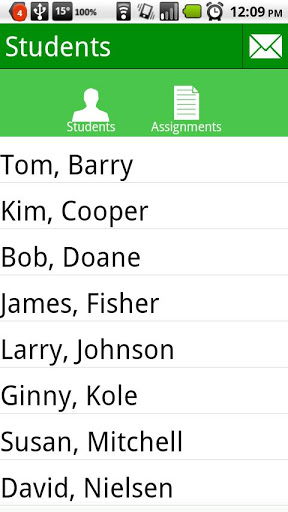
\includegraphics[scale=0.5]{grade_book01.jpg}
        \caption{Grade Book}
        \label{fig:Grade Book}
    \end{center}
\end{figure}

\subsection{Attendance}
https://play.google.com/store/apps/details?id=com.academics.attendance
Attendance

A great way to take attendance. Put your student list in a Google Spreadsheet, and this app takes care of the rest. There is no need to enter total absences into a spreadsheet at the end of the semester because all absences/tardies are calculated in your google spreadsheet each day you take attendance.

HOW-TO on website: http://androidforacademics.com/2010/09/attendance-instruction-manual/

Keywords: attendance
Price: Free
\begin{figure}
    \begin{center}
        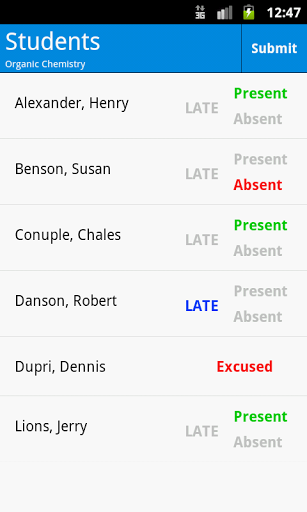
\includegraphics[scale=0.5]{attendance01.png}
        \caption{Attendance}
        \label{fig:Attendance}
    \end{center}
\end{figure}




\subsection{ Teacher Organizer }

https://play.google.com/store/apps/details?id=com.sorokinkirill.teacherorganizer
Gradebook and attendance, notes, schedule a teacher (high school teacher)

Unified information resource teacher developed within diploma projects.

Implemented the following functionality:
1. functional log attendance and log evaluations point system of evaluation, while allowing classes to celebrate and stand missing the mark;
1.1. compilation of the magazine is "on the fly", depending on the selected students;
1.2. selection of students by selecting a training group, not the individual student;
1.3. Log open it is possible to select more than one group of students;

2. entering information about your child and watching it like when viewing the log evaluations or visits, and without the need to open the log;

3. notebook;
3.1. notebook allows you to store notes, view, and edit;
3.2. a system for cataloging notes for quick search;
3.3. The possibility of entering one note in more than one subject group;

4. schedule a private teacher;
4.1. it is possible to view the schedule for the next semester as up to now, and after;
4.2. the system can generate the schedule for a few weeks in advance, if it is repeated;
4.3. supports two-week schedule (odd and even weeks).

Home Page: http://4pda.ru/forum/index.php?showtopic=345457\&st=80
Program in Russian

Price : Free
This seems to be very professional.

\begin{figure}
    \begin{center}
        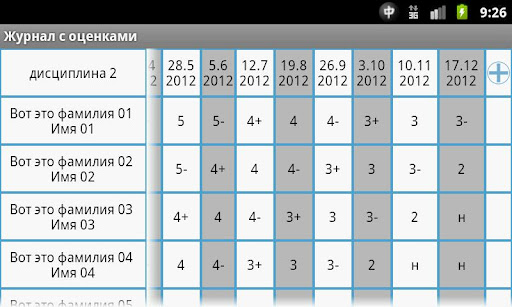
\includegraphics[scale=0.5]{teacher_organizer01.jpg}
        \caption{Teacher Organizer}
        \label{fig:TeacherOrganizer}
    \end{center}
\end{figure}





\subsection{Teacher Aide  }

https://play.google.com/store/apps/details?id=com.glen.apps.TeacherAideProLite

This is a free DEMO version of the Teacher Aide Pro app. The app allows teachers to take attendance and record grades on their phone or tablet. The main features are listed below.

The Lite version only allows the user to keep data for 5 students per class - otherwise all functionality is present so the user can truly test out the app before purchasing the PRO version

Features
- default values set to Present for fast attendance
- import student names via CSV file
- export data via CSV generated file send via email or to Dropbox (THE CLOUD)
- 1-click text to students/parents for tardy/absent students and missing assignments.
- 1-click Random student generator (no more popsicle sticks)
- Grading interface to allow recording of assignments using Yes/No/Missing, Points, Letter Grades, Percent.
- Generate PDF file for attendance and grade reports.
- Print reports directly to Google Cloud Printer from app.

New Features added all the time.

Explanation for some Permissions
SMS-Allows user to send bulk text message to parents and students
CALL Phone - Call parents/student right from the App
INTERNET - Send bulk email to parents/students from app without having to confirm 1 at a time
READ CONTACTS - Allows the user to save or load student/parent contacts from the device contact list. Your contact data is not read FOR ANY OTHER REASON, NOR TRANSMITTED OVER THE INTERNET.

I am a high school science teacher in the San Francisco Bay area.
Feedback or to inpocketsolution@gmail.com

Keywords: Attendance, Teacher, School, Roster, SIS, Gradebook, grades, TA, Teacher assistant, professor, coaches, team, sport, grading, gradebook, gradebook, schoolloop



Excellent but not free.

\begin{figure}
    \begin{center}
        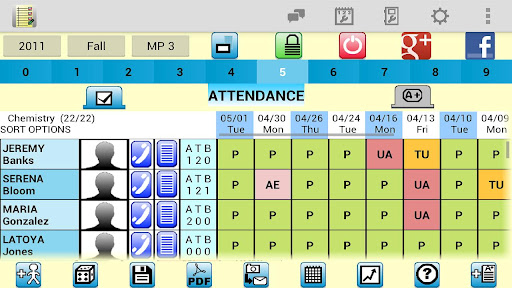
\includegraphics[scale=0.5]{TeacherAideProLite01.jpg}
        \caption{Teacher Aide}
        \label{fig:TeacherAide}
    \end{center}
\end{figure}




Bas�ndose en art�culos, libros, etc. que se os haya facilitado y
de otros que estim�is oportuno, se hablar� de:
\section{Descripci�n del problema}
\dots
\section{Descripci�n de los trabajos anteriores que se han dedicado a resolverlo}
\dots
